\documentclass[class=book, crop=false, oneside, 12pt]{standalone}
\usepackage{standalone}

\usepackage{../../style}
\usepackage{../../style_tree}

\graphicspath{{./assets/images/}}

\begin{document}
\chapter{Le grammatiche generative}

\section{Definizione di grammatica generativa}
Le grammatiche che tratteremo in questo corso sono chiamate grammatiche generative (così dette perché vengono usate per generare linguaggi).

Il primo passo per definire una grammatica è definirne il vocabolario, questo consiste in un set di simboli.
Alcuni di questi simboli sono chiamati terminali (terminals) e giocano il ruolo di token nell’analisi lessicale.
Un simbolo particolare nella grammatica è lo starting symbol: come suggerisce il nome, questo è il simbolo che permette di iniziare a generare il linguaggio derivato dalla grammatica (tale processo sarà chiarito in seguito).

Altra cosa da fissare in una grammatica è il set delle produzioni (productions); queste sono regole di riscrittura da stringhe ad altre stringhe e rispettano la seguente limitazione: la stringa di partenza deve contenere almeno un simbolo non-terminale.

Un esempio di regole per una grammatica è il seguente:
\begin{equation}
    \{S \to aSb, S \to ab\}
    \label{produzioni_esempio_0}
\end{equation}
Dove \(S\) è lo starting point mentre \(a\) e \(b\) sono caratteri terminali (a volte detti anche parole).\\
Per quanto abbiamo visto fin ora una grammatica generativa è composta da:
	\begin{itemize}
        \item Un vocabolario, ovvero l'insieme dei simboli
        \item Alcuni simboli speciali, ovvero i terminali, i non terminali ed il simbolo di partenza
        \item Le produzioni, ovvero regole che permettono di trasformare stringhe contenenti non terminali in qualcos’altro
    \end{itemize}
Questi sono gli ingredienti di una grammatica generativa.

Il linguaggio di una grammatica è l’insieme di stringhe composte solo da terminali che può essere generato partendo dallo starting point di quella stessa grammatica.

\subsection{Derivare il linguaggio di una grammatica generativa}
Per derivare un linguaggio dalla grammatica generativa dobbiamo applicare (quante volte possiamo) tutte le regole di riscrittura che appartengono alla grammatica stessa.\\
Ogni riscrittura è chiamata derivation step (simbolo \(\implies\), diverso dal simbolo usato nelle produzioni \(\to\)).
L’operazione di derivazione serve per tradurre stringhe con caratteri non terminali in stringhe composte solo da caratteri terminali (seguendo le regole dettate dalle produzioni).


Continuiamo con il nostro esempio:\\
Partendo dalla grammatica espressa in \ref{produzioni_esempio_0} possiamo sviluppare la seguente derivazione:
\begin{equation}
    S \implies ab
\end{equation}
Questa è una derivazione da \(S\) con un singolo step; la parola \(ab\) appartiene al linguaggio della nostra grammatica d’esempio.
Un'altra derivazione possibile è la seguente:
\begin{equation}
    S \implies aSb \implies aaSbb
\end{equation}
Diversamente da prima, \(aaSbb\) non è una parola del linguaggio perché non è composta \emph{solo} da caratteri terminali.

In questo modo si può definire qual è il linguaggio determinato da una grammatica, ad esempio con la grammatica che abbiamo visto prima possiamo generare ogni sequenza di parole formate da \(n\) terminali \(a\) seguiti da \(n\) terminali \(b\).
Tale linguaggio può essere scritto formalmente in questo modo:
\begin{equation}
    \{a^n b^n \mid n>0\}
\end{equation}


L'utilità del meccanismo di derivazione del linguaggio può esserci più chiara se pensiamo all'esempio appena visto come un metodo per verificare che tutte le parentesi aperte vengano chiuse, dove il terminale \(a\) sta per parentesi aperta ed il terminale \(b\) sta per parentesi chiusa. Una grammatica come \ref{produzioni_esempio_0} tramite il mezzo delle produzioni ci permette di eseguire questo tipo di controlli.

\paragraph{Regole di notazione}
Presentiamo ora alcune regole di notazione per lavorare con il processo di derivazione delle grammatiche generative.
\begin{itemize}
    \item i simboli del vocabolario prescelto che non fungono da terminali verranno sempre indicati con lettere maiuscole
    \item il carattere \(\varepsilon\) denota la parola vuota
    \item la lunghezza di \(\varepsilon\) è zero
    \item \(\varepsilon\) = \(\varepsilon\)\(\varepsilon\)
    \item \(\varepsilon\) =  \(b^0\) dove \(b\) è un qualunque carattere terminale
    \item il carattere \(\varepsilon\) non viene scritto nelle parole
\end{itemize}

\section{Esercizi di derivazione da una grammatica}
Presentiamo ora una serie di esercizietti di derivazione del linguaggio da una certa grammatica, con breve spiegazione del processo.

\begin{table}[H]
	\centering
	\subimport{assets/tables/}{exercise1.tex}
    \caption{Esercizio 1}
    \label{Esercizio 1}
\end{table}
\subsubsection*{Spiegazione di \ref{Esercizio 1}:}
Ricordiamo che si parte sempre e solo dallo starting symbol a derivare un linguaggio, quindi da \(S\).

L'unica derivazione che si può effettuare in questo caso è \(S \implies aAb\).
Da qui in poi non si può procedere che con una delle due productions \(aA \to aaAb\) oppure \(A \to \varepsilon\), in un caso si aumenterà la stringa di un \(a\) a sinistra e di un \(b\) a destra, nell'altro caso si terminerà la derivazione.

Diventa quindi semplice vedere che il linguaggio di questa grammatica è lo stesso generato da \ref{produzioni_esempio_0}, ovvero: \(\{a^n b^n \mid n>0\}\).

\begin{table}[H]
	\centering
	\subimport{assets/tables/}{exercise2.tex}
    \caption{Esercizio 2}
    \label{Esercizio 2}
\end{table}
\subsubsection*{Spiegazione di \ref{Esercizio 2}:}
Come prima si parte dal simbolo \(S\) che anche questa volta ci permette una sola produzione, quindi deriviamo senza ulteriori indugi: \(S \implies AB\).

In seguito ci rendiamo conto che le productions dell'esercizio altro non sono che delle regole per generare un numero a nostro piacimento di terminali \(a\) e \(b\), quindi deriviamo tranquillamente il seguente linguaggio: \(\{a^n b^m \mid n,m>1\}\).

\begin{table}[H]
	\centering
	\subimport{assets/tables/}{exercise3.tex}
    \caption{Esercizio 3}
    \label{Esercizio 3}
\end{table}
\subsubsection*{Spiegazione di \ref{Esercizio 3}:}
In questo caso il simbolo di partenza \(S\) ci offre due possibili productions, quindi dobbiamo sperimentarle entrambe per generare il linguaggio completo.

La seconda produzione ci porta subito ad una derivazione terminale \(S \implies abc\).
La prima produzione invece \(S \to aSBc\) ci permette di ricorrere in un processo ricorsivo che continua ad aggiungere terminali \(a\) sulla sinistra, la coppia \(Bc\) sulla destra e termina solo quando decidiamo di sostituire \(S\) con \(abc\).

Questo implica che nella situazione terminale ci potremo trovare in una situazione in cui abbiamo una stringa con questa forma \(aaa...abcBcBcBc...Bc\).

Da questa forma per eliminare tutti i non terminali \(B\) non abbiamo altra soluzione se non quella di utilizzare la produzione \(cB \to Bc\) per spostare tutte le \(c\) in fondo ed in seguito con \(bB \to bb\) trasformare tutte le \(B\) in \(b\).

Il linguaggio che ricaviamo alla fine è \(\{a^nb^nc^n \mid n>0\}\).

\begin{table}[H]
	\centering
	\subimport{assets/tables/}{exercise4.tex}
    \caption{Esercizio 4}
    \label{Esercizio 4}
\end{table}
\subsubsection*{Spiegazione di \ref{Esercizio 4}:}
La grammatica specificata nell'esercizio non permette di generare stringhe contenenti solo caratteri terminali, di conseguenza non genera alcuna parola valida.

Essendo il linguaggio definito come un insieme di parole che la grammatica può creare, per male che vada tale insieme è vuoto, ma esiste sempre. Questo è proprio il nostro caso, il linguaggio di questa grammatica è l’insieme vuoto.

\begin{table}[H]
	\centering
	\subimport{assets/tables/}{exercise5.tex}
    \caption{Esercizio 5}
    \label{Esercizio 5}
\end{table}
\subsubsection*{Spiegazione di \ref{Esercizio 5}:}
Non c'è molto da dire in questo caso se non che l’insieme contenente la parola vuota è diverso dall’insieme vuoto \(\{\varepsilon\} \neq \Phi\).

\begin{table}[H]
	\centering
	\subimport{assets/tables/}{exercise6.tex}
    \caption{Esercizio 6}
    \label{Esercizio 6}
\end{table}
\subsubsection*{Spiegazione di \ref{Esercizio 6}:}
La spiegazione è lasciata al lettore.

\begin{table}[H]
	\centering
	\subimport{assets/tables/}{exercise7.tex}
    \caption{Esercizio 7}
    \label{Esercizio 7}
\end{table}
\subsubsection*{Spiegazione di \ref{Esercizio 7}:}
Prima di tutto partiamo da \(S\), l'unica produzione possibile ci porta a \(CD\); ora possiamo dimenticarci di \(S\).

Vediamo subito che sia \(C\) che \(D\) possono essere trasformate in \(\varepsilon\) a piacimento, quindi possiamo interrompere le derivazioni da loro in ogni momento.

Ora, \(C\) ci permette di utilizzare le due produzioni \(C \to aCA\) e \(C \to bCB\) (il simbolo \(\mid\) ci dice che da \(C\) posso produrre \(sCA\) \emph{or} \(bCB\)).

Notiamo che se siamo in una forma del tipo \(aCAD\) possiamo proseguire con le produzioni di \(C\) oppure possiamo utilizzare \(AD \to aD\) ed osservando bene notiamo che questo è l'unico modo in cui potremo eliminare il non terminale \(A\), il che è speculare per quanto riguarda il caso \(bCBD\).

Notiamo inoltre che per ogni nuovo non terminale che aggiungiamo sulla destra dovremo farlo scorrere fino al limite estremo destro della parola (dove si trova \(D\)) per trasformarlo in terminale; a questo aggiungiamo che per ogni \(a\) sulla sinistra aggiungo \(A\) sulla destra ed in egual modo funziona per \(b\).

Ora dovrebbe essere chiaro che, al termine delle derivazioni, il numero di \(a\) sulla sinistra  sarà uguale al numero di \(a\) sulla destra e lo stesso per \(b\); inoltre al non terminale appena a sinistra dell'ultimo \(C\) corrisponderà un terminale uguale in posizione estrema destra (appena prima di \(D\)).

La soluzione è quindi \(\{ ww \mid w \in \{a^* b^*\}^*\}\).

\section{Grammatiche Generative formalmente}
Una grammatica generativa è una tupla con questa forma \(\mathcal{G}=(V, T, S, P)\):
\begin{itemize}
    \item \(V\) è il vocabolario (simboli terminali e non, completo)
    \item \(T\) è il set dei simboli terminali
    \item \(S\) è lo start symbol
    \item \(P\) è il set delle produzioni
\end{itemize}
Una volta definiti i componenti di una grammatica generativa, definiamo le convenzioni notazionali (o notazioni convenzionali) che si usano in questo campo:
\begin{itemize}
    \item Lettere maiuscole all’inizio dell’alfabeto (\(A\), \(B\)…) significano simbolo non terminale (\(\in (V \setminus T)\)).
    \item Lettere maiuscole alla fine dell’alfabeto (\(X\), \(Y\), \(Z\)…) un generico simbolo del vocabolario, terminale o meno, non si sa (\(\in V\)).
    \item Lettere minuscole inizio alfabeto (\(a\), \(b\)…) per indicare caratteri terminali (\(\in T\)).
    \item Lettere minuscole greche per indicare stringhe che possono essere composte da terminali o non terminali \(\in V^*\), dove \(^*\) significa che possono esserci zero o più ripetizioni di elementi nella base.
    \item Lettere minuscole in fondo all’alfabeto con pedice numerico (\(w\), \(w_0\)…) per indicare stringhe di caratteri terminali
\end{itemize}
Definiamo ora formalmente l'oggetto produzione, esso è una traduzione in questa forma:
\begin{equation}
    \delta \to \beta
\end{equation}
Dove \(\delta \in V^+\), \(\delta\) contiene almeno un non terminale (non traduciamo terminali in altri terminali); il \(^+\) significa che c’è una o più ripetizioni di elementi nella base, che quindi non è vuota (\(\varepsilon\)).\\
\(\delta\) è detto \textbf{driver} della produzione mentre \(\beta\) è detto \textbf{corpo} della produzione.

Il linguaggio generato da una grammatica \(\mathcal{G} = (V,T,S,P)\) è così definito:
\begin{equation}
    \mathcal{L}(\mathcal{G}) = {w \mid w \in T^* and \; S \implies^* \; w }
\end{equation}
Ovvero l'insieme di tutti gli elementi (anche vuoti) che si possono derivare con uno o più passi dallo starting point.

\subsection{Tipi di grammatiche generative}
Esiste una gerarchia delle grammatiche, che non dipende dal genere di analisi che permettono di fare, ma dipende solo dalla struttura delle loro produzioni.

Si parla di Context-free grammars, o free grammars, quando tutte le produzioni sono in forma \(A \to \beta\), ovvero che hanno driver composti \emph{solo} da non terminali.

Queste grammatiche sono molto importanti perché praticamente tutti i linguaggi di programmazione sono derivati da questo tipo di grammatica.
Si dice di un linguaggio che è context-free se esiste una grammatica libera che genera quello steso linguaggio.
\(\mathcal{L}\) è un linguaggio libero se e solo se esiste una grammatica libera \(\mathcal{G}\) tale che \(\mathcal{L}=\mathcal{L}(\mathcal{G})\).

L’operazione di analizzare una stringa e verificare se appartiene ad una determinata grammatica dipende naturalmente dal metodo con cui si decide di applicare la derivazione dallo starting point della grammatica stessa.

Se una stringa si può derivare da una certa grammatica, si dice che la prima appartiene al linguaggio di quest'ultima.
Esistono due tipi di derivazione canonica:
\begin{itemize}
    \item Rightmost (si rimpiazzano sempre prima i non terminali più a destra)
    \item Leftmost (si rimpiazzano sempre prima i non terminali più a sinistra)
\end{itemize}
Se utilizziamo come strategia una di queste due tutti i passi analitici di una derivazione sono deterministici, perché ad ogni passo o procedo con l’elemento più a destra o procedo con quello più a sinistra. Per questo motivo queste sono le due modalità di derivazione canonica.

Le grammatiche libere si prestano in modo naturale ad essere processate tramite il cosiddetto albero di derivazione.
Questo albero ha come radice lo starting point, poi, per ogni passo di derivazione secondo una produzione in forma \(A \to X_1 \mid X_2 \mid\dots\mid X_n \), si generano \(n\) figli del nodo con la derivazione di \(A\) messa in atto.
Le foglie dell’albero saranno composte da \(\varepsilon\) oppure da caratteri terminali. In figura \ref{albero_di_derivazione} è riportato come esempio l'albero di derivazione della grammatica:
\begin{equation}
    S \to aSb \mid \varepsilon
    \label{grammatica_allbero}
\end{equation}

\begin{figure}[H]
	\centering
    \subimport{assets/figures/}{albero-derivazione1.tex}
    \caption{Albero di derivazione di \ref{grammatica_allbero}}
    \label{albero_di_derivazione}
\end{figure}
Ma tornando con i piedi per terra, cosa centra tutto questo con i compilatori?\\
Un certo programma che è stato trasformato in una stringa viene verificato controllando che la tale stringa sia derivata dalla grammatica del linguaggio in cui il programma è scritto. Un modo per verificare questo è trovare l’albero di derivazione della stringa che rappresenta il tal programma.

\subsection{Ambiguità delle grammatiche}
Una grammatica \(\mathcal{G}\) si dice ambigua se esiste \(w \in \mathcal{L}(\mathcal{G})\) che può essere derivata da due derivazioni canoniche distinte, entrambe rightmost o entrambe leftmost. Distinte significa che l'ordine di applicazione delle produzioni è differente, ma questo sarà più chiaro in seguito.

Noi non vogliamo grammatiche ambigue, ci complicano la vita.
Prendiamo ad esempio la grammatica delle espressioni aritmetiche:
\begin{equation}
    E \to E+E \mid E*E \mid  n
\end{equation}
Intuitivamente si può leggere come exp -> exp+exp  o  exp*exp  o  numero.\\
Questa grammatica ci permette di fare operazioni di somma o moltiplicazione, è ambigua o meno?

Per verificarlo proviamo a derivare questo \(w = n+n*n\) utilizzando la tecnica leftmost e generando due derivazioni distinte.

\begin{figure}[H]
	\centering
	\subimport{assets/figures/}{derivazione-leftmost.tex}
    \caption{Derivazione leftmost 1}
    \label{leftmost_1}
\end{figure}
Nel primo caso di derivazione leftmost (\ref{leftmost_1}) partiamo con il trasformare \(E\) in \(E+E\); di seguito proseguendo in leftmost trasformiamo la prima \(E\) in \(n\), poi la seconda \(E\) in \(E*E\).
Infine trasformiamo (sempre da sinistra a destra) entrambe le \(E\) rimanenti in \(n\).

Semplice, no? Ora proviamo ad ottenere la stessa parola in modo alternativo:
\begin{figure}[H]
	\centering
	\subimport{assets/figures/}{derivazione-righmost.tex}
    \caption{Derivazione leftmost 2}
    \label{leftmost_2}
\end{figure}
Si nota subito che la differenza sostanziale è che in questo secondo caso (\ref{leftmost_2}) la prima produzione che utilizziamo non è \(E \to E+E\), bensì \(E \to E*E\).

Questo comporta due derivazioni differenti anche se entrambe sono nella stessa forma canonica leftmost.
La grammatica di partenza è quindi ambigua: nonostante il significato (l'interpretazione matematica dei due alberi) sia diverso riusciamo a costruire \(w\) con due alberi differenti che usano la stessa strategia canonica di derivazione.

Ora abbiamo visto questo processo, sappi che la prof.ssa Quaglia preferisce 14 a 1 la derivazione con albero a quella con stringa perché è più chiara.

\subsubsection*{Dangling Else}
Introduciamo una nuova forma di grammatica
\begin{equation}
    S \to \; if \; b \; then \; S |\; if\; B\; then\; S\; else\; S |\; other
\end{equation}
È una grammatica ambigua?

Prendiamo ad esempio questa parola:
\begin{equation}
    \label{dangling_else}
    w =\; if\; b\; then\; if\; b\; then\; other\; else\; other
\end{equation}
Con quale \(then\) è accoppiato l’\(else\)? Non si può sapere!

Di fatto possiamo ricostruire \(w\) con questi due diversi alberi:
\begin{figure}
	\centering
    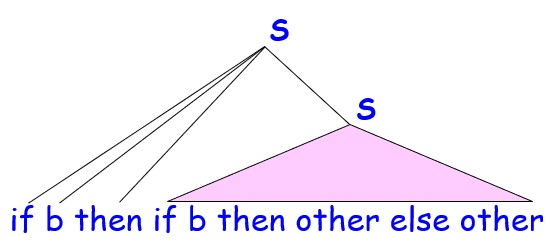
\includegraphics[width=.7\textwidth,keepaspectratio]{dangling_else_1.jpg}
    \caption{Primo albero di derivazione per Eq. \ref{dangling_else}}
    \label{dangling_else_1}
\end{figure}
\begin{figure}
	\centering
    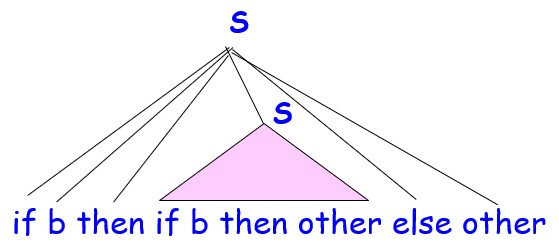
\includegraphics[width=.7\textwidth,keepaspectratio]{dangling_else_2.jpg}
    \caption{Secondo albero di derivazione per Eq. \ref{dangling_else}}
    \label{dangling_else_2}
\end{figure}
Questo ci introduce il problema di come trattare la gestione del comando \(if \; then \; else\) in un linguaggio di programmazione.
Per questo nei vari linguaggi troviamo sempre qualche forma di strategia per risolvere questo problema:
\begin{itemize}
    \item Mettere le parentesi
    \item Eliminare l’else e usare solo if
    \item Usare la regola del closest unmatched then (l’\(else\) è sempre valutato come appartenente all’ultimo \(then\) non ancora elsato)
\end{itemize}
L’else è intrinsecamente ambiguo.

Osservazione:\\
L’ambiguità in alcuni casi può essere indecidibile, in quanto non sempre esiste un algoritmo che ci dice se la grammatica è ambigua o no.

\subsection{Piccola parentesi sui linguaggi naturali}
I linguaggi naturali spesso nascondono molte più ambiguità delle grammatiche che affronteremo in questo corso.
D'altro canto le grammatiche per linguaggi di programmazione sono molto difficili da scrivere anche perché sono pensate e studiate per ottenere una certa velocità di verifica dei programmi.
Il linguaggio naturale è ben più complesso: immagina quanto dev’essere difficile descrivere una grammatica per il linguaggio naturale ed immagina poi quale complessità può avere un algoritmo di verifica di tale grammatica, ammesso che questo possa esistere.

Pensa solo al fatto che spesso e volentieri il linguaggio naturale dipende dal contesto! Questa cosa nei linguaggi di programmazione non s’è mai vista per fortuna.

I parser per linguaggi di programmazione hanno complessità lineare di norma, se si va a vedere i parser del linguaggio naturale\dots  sayonara!

\end{document}
